\mode*

\section{Listor}

\begin{frame}[fragile]
  \mintinline[fontsize=\huge,escapeinside=||]{python}{var = [item0, |$\dotsc$|, itemN]}
\end{frame}

\begin{frame}[fragile]
  \begin{example}
    \begin{minted}{python}
names = ["Adam", "Bertil", "Cesar"]
print(names[0])
print(names[1])
print(names[2])
print(names[3])
    \end{minted}
  \end{example}

  \pause

  \begin{example}
    \begin{minted}{python}
numbers = [2, 3, 12, 3, 12, 12]
print(numbers[0])
print(numbers[1])
print(numbers[2])
    \end{minted}
  \end{example}
\end{frame}

\begin{frame}
  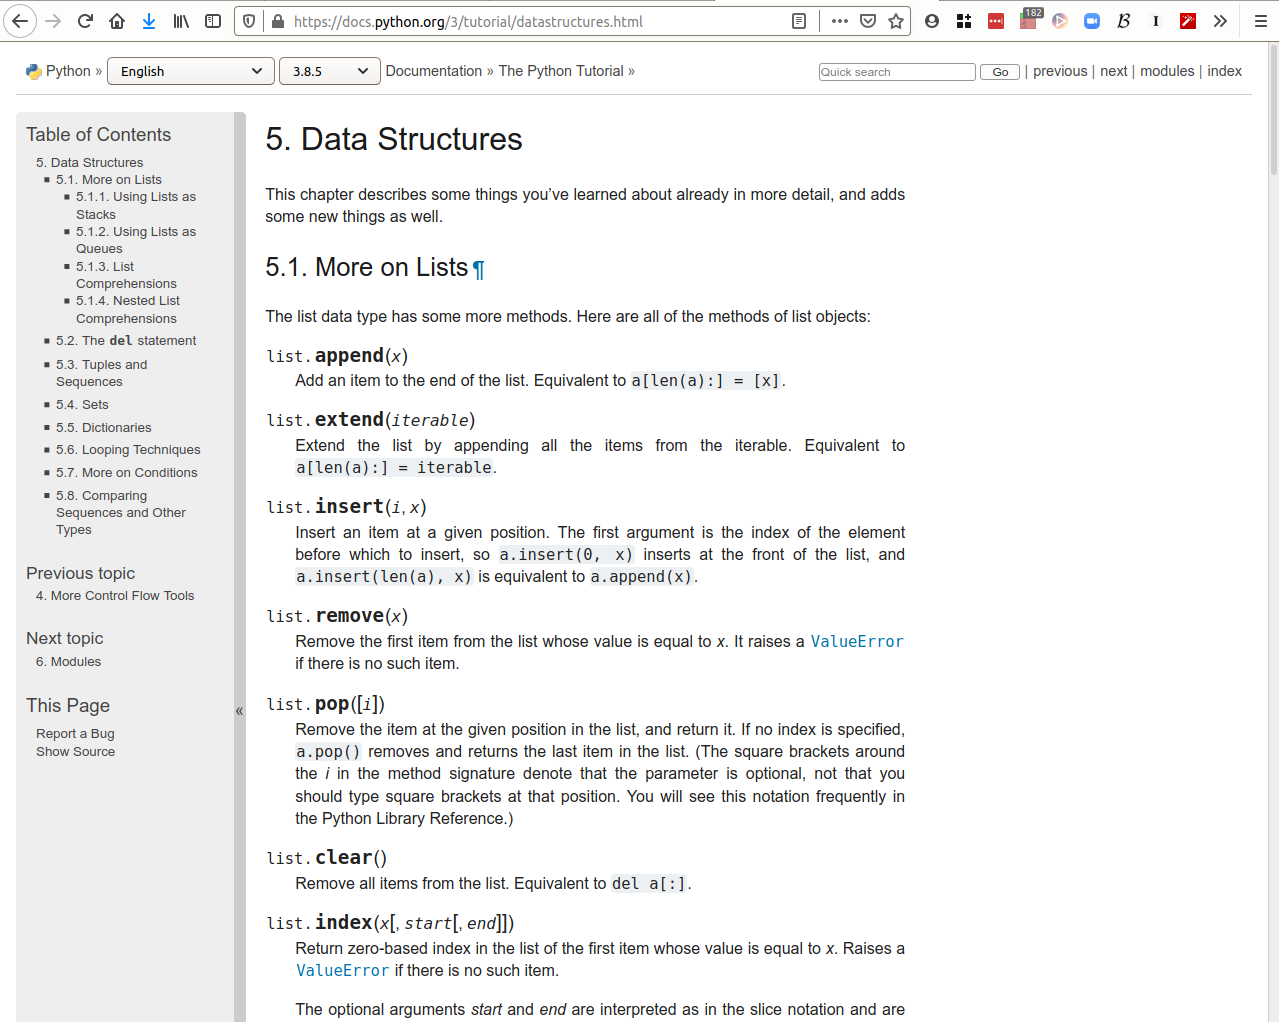
\includegraphics[width=\columnwidth]{figs/docs-lists.png}
\end{frame}

\begin{frame}[fragile]
  \begin{example}[extend\textunderscore{}lists.py]
    \inputminted{python}{examples/extend_lists.py}
  \end{example}
\end{frame}

\begin{frame}[fragile]
  \begin{exercise}[input\textunderscore{}list.py]
    \begin{itemize}
      \item Skriv ett program (modul med testprogram) som läser in namn och 
        lägger i en lista.
    \end{itemize}
  \end{exercise}
\end{frame}

\begin{frame}[fragile]
  \begin{example}
    \begin{minted}{python}
names = ["Adam", "Bertil", "Cesar"]
names[0] = "Ada"
names[1] = "Beda"
names[2] = "Cissi"
print(names[0])
print(names[1])
print(names[2])
names[3] = "Diddi"
    \end{minted}
  \end{example}
\end{frame}

\begin{frame}[fragile]
  \begin{example}
    \begin{minted}{python}
names = ["Adam", "Bertil", "Cesar"]
print(f"Det finns {len(names)} namn i listan {names}")
    \end{minted}
  \end{example}
\end{frame}

\begin{frame}[fragile]
  \begin{example}[Aritmetiska \emph{hel}talsföljder]
    \begin{minted}{python}
print(list(range(10)))
print(list(range(0, 10)))
print(list(range(1, 10, 2)))
    \end{minted}
  \end{example}
\end{frame}


\section{Iterationer med for-slingor}

\begin{frame}[fragile]
  \begin{minted}[fontsize=\huge,numbers=none]{python}
for item in container:
  print(item)
  \end{minted}
\end{frame}

\begin{frame}[fragile]
  \begin{example}
    \begin{minted}{python}
for i in range(10):
  print(i)
    \end{minted}
  \end{example}

  \pause

  \begin{example}
    \begin{minted}{python}
for person in ["adam", "bertil", "cesar"]:
    print(person)
    \end{minted}
  \end{example}

  \pause

  \begin{example}
    \begin{minted}{python}
names = ["adam", "bertil", "cesar"]
for index in range(len(names)):
    print(names[index])
    \end{minted}
  \end{example}
\end{frame}

\begin{frame}[fragile]
  \begin{exercise}[modlist.py]
    \begin{itemize}
      \item Skriv ett program som läser in namn och lägger i en 
        lista.
      \item Skriv ut listan numrerad, låt användaren välja vilket element som 
        ska ändras.
      \item Låt användaren mata in ett nytt värde för indexet.
    \end{itemize}
  \end{exercise}
\end{frame}

\subsection{Skapa en lista från annan lista}

\begin{frame}[fragile]
  \mintinline[fontsize=\huge]{python}{var = [f(x) for x in lst]}
\end{frame}

\begin{frame}[fragile]
  \begin{example}[List comprehensions]
    \begin{minted}{python}
squares = [x**2 for x in range(10)]
    \end{minted}
  \end{example}

  \pause

  \begin{example}[List comprehensions]
    \begin{minted}{python}
names = ["anna", "cissi"]
names_capitalized = [name.capitalize() for name in names]
    \end{minted}
  \end{example}
\end{frame}


\section{Sökning, sortering mm}

\subsection{Sökning}

\begin{frame}[fragile]
  \mintinline[fontsize=\huge]{python}|item in list|
\end{frame}

\begin{frame}[fragile]
  \begin{example}[isin.py]
    \inputminted{python}{examples/isin.py}
  \end{example}
\end{frame}

\begin{frame}[fragile]
  \begin{exercise}[search.py]
    \begin{itemize}
      \item Skriv ett program som låter oss mata in ett antal 
        namn.
      \item Därefter får vi söka bland namnen.
    \end{itemize}
  \end{exercise}
\end{frame}

\begin{frame}[fragile]
  \begin{exercise}[search.py]
    \begin{itemize}
      \item Skriv ett program som låter oss mata in ett antal 
        namn.
      \item Därefter får vi söka bland namnen.
    \end{itemize}
  \end{exercise}

  \begin{exercise}[partial\textunderscore{}search.py]
    \begin{itemize}
      \item Ändra programmet så att vi kan söka efter delar av namn.
%      \item Tips: testa hur \mintinline{python}|in| funkar på strängar; 
%        \mintinline{python}|"kaka" in "pepparkaka"|.
    \end{itemize}
  \end{exercise}
\end{frame}

\subsection{Sortering}

\begin{frame}[fragile]
  \begin{example}[Sortering]
    \begin{minted}{python}
      names = ["Beda", "Ada", "Cissi"]
      print(sorted(names))
    \end{minted}
  \end{example}

  \begin{exercise}[Från OLI]
    \begin{itemize}
      \item Vad är förväntat resultat och varför?
    \end{itemize}
    \begin{minted}{python}
numbers = ["2", "1", "3"]
print(sorted(numbers))

numbers.extend(["13", "12", "11"])
print(sorted(numbers))
    \end{minted}
  \end{exercise}
\end{frame}

\begin{frame}[fragile]
  \begin{example}[Sortering]
    \begin{minted}{python}
      names = ["Beda", "Ada", "Cissi"]
      print(sorted(names, key=len))
    \end{minted}
  \end{example}

  \begin{exercise}
    \begin{itemize}
      \item \mintinline{python}|sorted| kan sortera på andra sätt också, läs 
        \mintinline{bash}|pydoc3 sorted|.
      \item Vad gör koden i exemplet ovan?
      \item Ändra sorteringen från stigande till sjunkade ordning.
    \end{itemize}
  \end{exercise}
\end{frame}

\subsection{Liknande funktioner}

\begin{frame}[fragile]
  \begin{example}
    \begin{minted}{python}
      names = ["Beda", "Ada", "Cissi"]
    \end{minted}
  \end{example}

  \begin{exercise}
    \begin{itemize}
      \item Plocka ut elementet ur \mintinline{python}|names| som är först 
        alfabetiskt.
      \item Plocka ut elementet ur \mintinline{python}|names| som är 
        längst.
    \end{itemize}
  \end{exercise}
\end{frame}

\begin{frame}[fragile]
  \begin{example}
    \begin{minted}{python}
      names = ["Beda", "Ada", "Cissi"]
    \end{minted}
  \end{example}

  \begin{exercise}
    \begin{itemize}
      \item Vad gör funktionerna \mintinline{python}|min| och 
        \mintinline{python}|max|?
      \item Plocka ut elementet ur \mintinline{python}|names| som är först 
        alfabetiskt.
      \item Plocka ut elementet ur \mintinline{python}|names| som är 
        längst.
    \end{itemize}
  \end{exercise}
\end{frame}
